\documentclass[../main.tex]{subfiles}
\graphicspath{{\subfix{../Images/}}}
\begin{document}


\subsection{Изучение сходимости интеграла $\int_{10}^\infty \frac{dx}{x^\alpha (\ln x)^\beta}$}
Рассмотрим случаи:\\\\
1. $\alpha > 1$: представим $\alpha = 1 + 2a$, $a > 0$, значит можно представить\\\\
выражение под интегралом в виде $\dfrac{1}{x^{\alpha} (\ln {x})^b} = \dfrac{1}{x^{1 + a}} \cdot \dfrac{1}{x^a(\ln{x})^{\beta}}$\\\\
Докажем, что $\lim\limits_{x \rightarrow +\infty} \dfrac{1}{x^a (\ln{x})^{\beta}} = 0$\\\\
Если $\beta \geq 0$, то всё ок. Если $\beta < 0$, то $\lim \dfrac{(\ln{x})^{-\beta}}{x^a} = \left( \lim \dfrac{\ln{x}}{x^{a / -\beta}} \right)^{-\beta} = 0$\\\\
Значит выражение под интегралом меньше или равно чем $\dfrac{1}{x^{1 + a}}$, а такой интеграл при $a > 0$ сходится\\\\\\
2. $\alpha < 1$, то $\alpha = 1 - 2 \gamma$, $\gamma > 0$\\\\
По аналогии, представим в виде произведения:\\
$\dfrac{1}{x^{1 - \gamma}} \cdot \dfrac{1}{x^{-\gamma}(\ln{x})^{\beta}} \geq \dfrac{1}{x^{1 - \gamma}}$\\\\
Выражение большее, чем несходящийся интеграл, значит расходится.\\\\\\
3. $\alpha = 1$, $\int\limits^{+\infty}_{10} \dfrac{dx}{x(\ln{x})^{\beta}} = \int\limits^{+\infty}_{10} \dfrac{dy}{y^{\beta}}$\\\\
$\beta > 1$ сходится, $\beta \leq 1$ расходится.\\\\\\\\

\newpage

\subsection{Интеграл Эйлера--Пуассона}
$\int\limits^{+\infty}_0 e^{-x^2} dx = \dfrac{\sqrt{\pi}}{2}$\\\\ \textbf{Доказательство:}\\\\
Рассмотрим функцию $\varphi(t) = \int\limits^t_0 e^{-x^2} dx$\\\\
Из неравенства $e^t \geq 1 + t$, при $t = x^2$ следует\\\\
$1 + x^2 \leq e^{x^2}$\\\\
$\dfrac{1}{1 + x^2} \geq \dfrac{1}{e^{x^2}}$\\\\
$1 - x^2 \leq e^{-x^2} \leq \dfrac{1}{1 + x^2}$\\\\
Интегрируем: $\int\limits^1_0 (1 - x^2)^n dx \leq \int\limits^1_0 e^{-nx^2} \leq \int\limits^{+\infty}_0 e^{-nx^2} \leq \int\limits^{+\infty}_{0} \dfrac{1}{(1 + x^2)^n} dx$\\\\
Левая часть: $x = \cos{t}$, тогда делаем замену и $\int\limits^0_{\pi / 2} \sin^{2n} {t} (-\sin{t}) dt = W_{2n + 1}$ ~--- формула Валлиса\\\\
Правая часть: $x = \tg {t}$ и $\dfrac{1}{1 + \tg^2{t}} = \cos^2{t}$\\\\
$\int\limits^{\pi / 2}_0 \cos^{2n} t \cdot \dfrac{1}{cos^2 t} dt = \int\limits^{\pi / 2}_0 \cos^{2n - 2} dt = W_{2n - 2}$\\\\
Средняя часть: $x = \dfrac{t}{\sqrt{n}}$ и $\sqrt{n} \int\limits^{+\infty}_0 e^{-t^2} dt$\\\\
$\sqrt{n} W_{2n + 1} \leq \int\limits^{+\infty}_0 e^{-x^2} dx \leq \sqrt{n} W_{2n - 2}$\\\\
$W_n = \dfrac{(n - 1)!!}{n!!}$\\\\
$W_{2n - 2} = \dfrac{(2n - 3)!!}{(2n - 2)!!} \cdot \sqrt{n} \cdot \dfrac{\pi}{2} = \dfrac{1}{\dfrac{(2n - 2)!!}{(2n - 3)!!} \dfrac{1}{\sqrt{n} - 1}} \cdot \dfrac{\sqrt{n}}{\sqrt{n} - 1} \cdot \dfrac{\pi}{2} = \dfrac{1}{\sqrt{\pi}} \cdot 1 \cdot \dfrac{\pi}{2} = \dfrac{\sqrt{\pi}}{2}$\\\\
$W_{2n + 1} = \dfrac{(2n)!!}{(2n + 1)!!} \cdot \sqrt{n} = \dfrac{(2n)!!}{(2n - 1)!!} \cdot \dfrac{1}{\sqrt{n}} \dfrac{n}{2n + 1} = \dfrac{\sqrt{\pi}}{2}$
\newpage


\subsection{Гамма функция Эйлера. Простейшие свойства.}
$\Gamma(T) = \int\limits^{+\infty}_0 x^{t - 1} e^{-x} dx$, $t > 0$ ~--- Гамма функция Эйлера\\\\\\
\textbf{Свойства:}\\\\
1. Интеграл сходится\\\\
2. Функция выпукла, значит она непрерывна\\\\
3. $\Gamma(t + 1) = t \Gamma (t)$\\\\
4. $\Gamma \left( \dfrac{1}{2} \right) = \sqrt{\pi}$\\\\
5. Парабола, вершина ~--- примерно точка $(1, 1)$, ветви полностью лежат в первой четверти\\\\
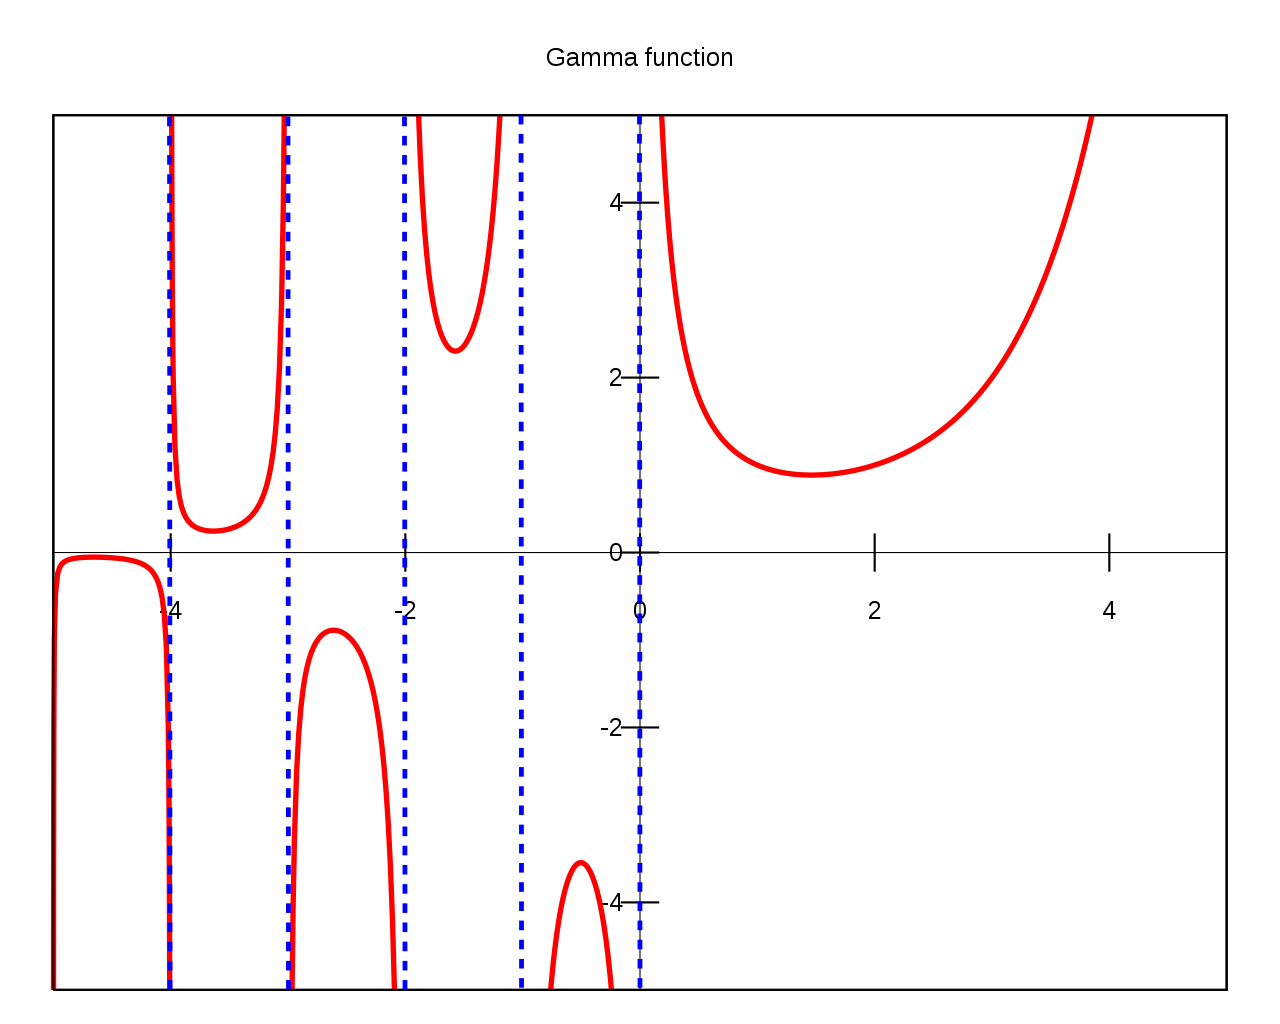
\includegraphics[scale = 0.2]{Images/gamma plot.png}\\\\
\newpage
\textbf{Доказательство:}\\\\
1. $\int\limits^{+\infty}_0 = \int\limits^1_0 + \int\limits^{+\infty}_1$\\
$\int\limits^1_0 x^{t - 1} e^{-x} dx$, при $x \rightarrow 0$ эквивалентно $x^{t - 1}$, $t > 1$, значит сходится\\\\
$\int\limits^{+\infty}_1 x^{t - 1} e^{-x} dx = \left( x^{t - 1} \cdot e^{-x / 2} \right) \cdot e^{-x / 2} \leq e^{-x / 2}$ при $x \geq x_0$, где $x_0 < 1$.\\\\
$\int\limits^{+\infty}_{x_0} e^{-x / 2} = \lim\limits_{B \rightarrow +\infty} \left(2 \cdot e^{-x_0 / 2} - 2 \cdot e^{-B / 2} \right)$ ~--- конечен\\\\\\
2. Подынтегральная функция $h : t \mapsto x^{t - 1} e^{-x}$ ~--- выпукла. \\\\
Продифференцируем $h'' = x^{t - 1} e^{-x} \ln^2{x} \geq 0$\\\\
$\forall x \in [0, 1] :  h \left(\alpha t_1 + (1 - \alpha) t_2, x \right) \leq \alpha h(t_1, x) + (1 - \alpha) h(t_2, x)$ ~--- неравенство Йенсена\\\\
$\Gamma(\alpha t_1 + (1 - \alpha) t_2) \leq \alpha \Gamma(t_1) + (1 - \alpha) \Gamma (t_2)$\\\\
$\Gamma(t)$ ~--- выпукла, значит она непрерывна\\\\\\
3. $\int\limits^{+\infty}_0 x^t e^{-x} dx = \begin{bmatrix} f = x^t & f' = t x^{t - 1} \\ g' = e^{-x} & g = -e^{-x} \end{bmatrix} = x^t(-e^{-x}) \bigg|^{+\infty}_0 + \int\limits^{+\infty}_0 t x^{t - 1} e^{-x} dx = t \Gamma(t)$\\\\
$\Gamma(1) = 1$, значит $\Gamma(n) = n!$\\\\\\
4. $\int\limits^{+\infty}_0 x^{-0.5} e^{-x} dx = 2 \int\limits^{+\infty}_0 e^{-y^2} dy$ ~--- интеграл Эйлера-Пуассона

\newpage

\subsection{Теорема об абсолютно сходящихся интегралах и рядах.}
Пусть $f$ ~--- допустима на $[a, b)$. Тогда эквивалентны утверждения:\\\\
1. $\int\limits^b_a f$ абсолютно сходится\\\\
2. $\int\limits^b_a |f|$ сходится\\\\
3. $\int\limits^b_a f^+$ и $\int\limits^b_a f^-$ абсолютно сходятся\\\\
\textbf{Доказательство}\\\\
$1 \Rightarrow 2$ ~--- очевидно\\\\
$2 \Rightarrow 3$ $0 \leq f^+ \leq |f|$ и $0 \leq f^- \leq |f|$\\\\
$3 \Rightarrow 1$ $f = f^+ - f^- \Rightarrow \int f$ ~--- сходится\\
$|f| = f^+ + f^- \Rightarrow \int |f|$ ~--- сходится\\\\
\textbf{Случай рядов}\\\\
Аналогично интегралам. Доказывается с помощью интегрального признака Коши.


\newpage


\subsection{Изучение интеграла $\int_1^{\infty} \frac{\sin x\,dx}{x^p}$ на сходимость и абсолютную сходимость}
Рассмотрим три случая:\\\\
1. При $p > 1 : \left| \dfrac{\sin{x}}{x^p} \right| \leq \dfrac{1}{x^p}$ ~--- абсолютная сходимость\\\\\\
2. При $p \leq 0 : \int\limits^{2 \pi k + \pi}_{2 \pi k} \dfrac{\sin{x}}{x^p} \geq \int\limits^{2 \pi k + \pi}_{2 \pi k} \sin{x} = 2$, значит интеграл расходится (и абсолютно тоже)\\\\\\
3.При $0 < p \leq 1$ нет абсолютной сходимости, но есть обычная сходимость:\\\\
$\int\limits^{+\infty}_1 \dfrac{\sin{x}}{x^p} = \begin{bmatrix} f' = \sin x & f = -\cos x \\ g = \dfrac{1}{x^p} & g' = -p \dfrac{1}{x^{p + 1}} \end{bmatrix} = - \cos{x} \cdot \dfrac{1}{x^p} \bigg|^{+\infty}_1 - p \int\limits^{+\infty}_1 \dfrac{\cos{x}}{x^{p + 1}} dx$ ~--- сходится\\\\\\
$\int\limits^{+\infty}_1 \dfrac{|\sin{x}|}{x^p} \geq \int\limits^{+\infty}_1 \dfrac{\sin^2 x}{x^p} = \dfrac{1}{2} \int\limits^{+\infty}_1 \left( \dfrac{1}{x^p} - \dfrac{\cos{2x}}{x^p} \right)$ ~--- расходится,т.к. $\int\limits^{+\infty}_1 \dfrac{1}{x^p}$ расходится, а $\int\limits^{+\infty}_1 \dfrac{\cos{2x}}{x^p}$ сходится.

\newpage


\end{document}